\documentclass[11pt]{article}
\usepackage{geometry}                % See geometry.pdf to learn the layout options. There are lots.
\geometry{letterpaper}                   % ... or a4paper or a5paper or ... 
%\geometry{landscape}                % Activate for for rotated page geometry
%\usepackage[parfill]{parskip}    % Activate to begin paragraphs with an empty line rather than an indent
\usepackage{graphicx}
\usepackage{amssymb,amsmath}
\usepackage{epstopdf}
\usepackage{pgf}
\usepackage{pgfpages}
\usepackage{tikz}
\usetikzlibrary{arrows,backgrounds}
\usepgflibrary{shapes}
\DeclareGraphicsRule{.tif}{png}{.png}{`convert #1 `dirname #1`/`basename #1 .tif`.png}
\pagestyle{empty}


\begin{document}

 \begin{center}
   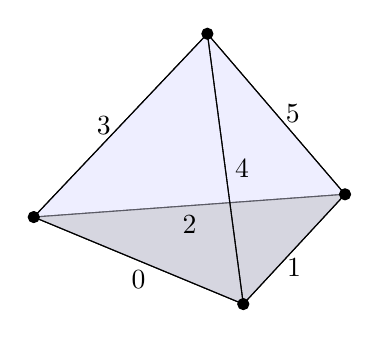
\begin{tikzpicture}[join=round] % Tetrahedron edges
        \filldraw[fill=blue!10,fill opacity=0.4](0,2.6)--(-2.205,.272)--(1.748,.561)--(0,2.6)--cycle;
        \filldraw[fill=black!20](1.748,.561)--(-2.205,.272)--(.456,-.833)--cycle;
        \filldraw[fill=blue!10,fill opacity=0.4](0,2.6)--(1.748,.561)--(.456,-.833)--(0,2.6)--cycle;
        \filldraw[fill=blue!10,fill opacity=0.4](0,2.6)--(.456,-.833)--(-2.205,.272)--(0,2.6)--cycle;
        \filldraw(1.748,.561) circle (2pt);
        \filldraw(-2.205,.272) circle (2pt);
        \filldraw(0,2.6) circle (2pt);
        \filldraw(.456,-.833) circle (2pt);
        \fill[black]
                (-.874,-.281) node [below] {0}
                (1.102,-.136) node [below] {1}
                (-.228,.417) node [below] {2}
                (-1.102,1.436) node [left] {3}
                (.228,.883) node [right] {4}
                (.874,1.581) node [right] {5};
   \end{tikzpicture}
  \end{center}
\end{document}  
